%% SW design: PSoC Controllers
\begin{figure}[htbp] \centering
{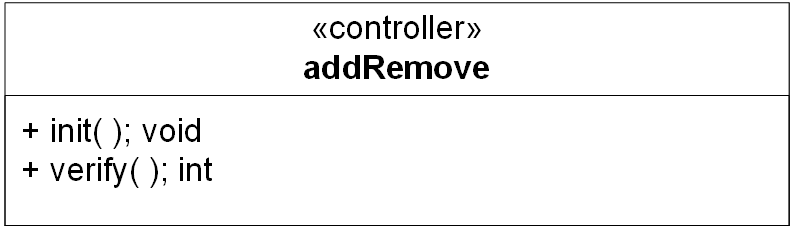
\includegraphics[scale=1.3]{filer/design/Klassediagrammer/sw_psoc_addRemove}}
\caption{Klasse addRemove}
\label{fig:sw_psoc_class_addremove}
\end{figure} 

{\centering
\textbf{addRemove}\par
}
\textbf{Ansvar:} Kontrollerer hændelsesforløbet ifm. usecase 1. \

\verb+int verify( )+\\
\textbf{Parametre:} Ingen \\
\textbf{Returværdi:} 0 ved succes ellers negativ i overenstemmelse med fejl-listen. \\
\textbf{Beskrivelse:} Returnerer kun 0. Bruges til at verificerer kommunikation mellem Master og Enhed.\\

\begin{figure}[htbp] \centering
{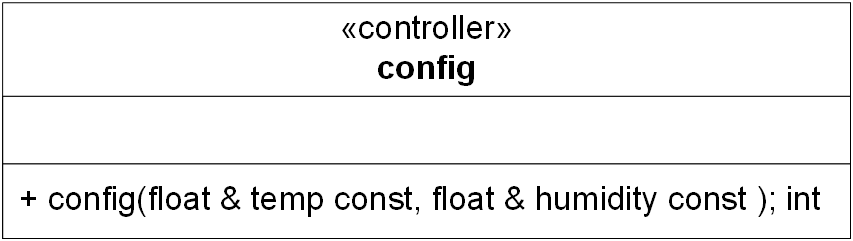
\includegraphics[scale=1.3]{filer/design/Klassediagrammer/sw_psoc_config}}
\caption{Klasse config}
\label{fig:sw_psoc_class_config}
\end{figure} 

{\centering
\textbf{config}\par
}
\textbf{Ansvar:} Kontrollerer hændelsesforløbet ifm. usecase 2. \

\verb+int config( const float * temp, const float * humidity  )+ \\
\textbf{Parametre:} To pointere til hhv. temperatur og fugtighedsgrænser \\
\textbf{Returværdi:} 0 ved succes ellers negativ i overenstemmelse med fejl-listen. \\
\textbf{Beskrivelse:} Skal gemme parametre i et objekt af typen parameters ved at kalde metoderne \verb+setTemp()+ og \verb+setHumi()+.\\

\begin{figure}[htbp] \centering
{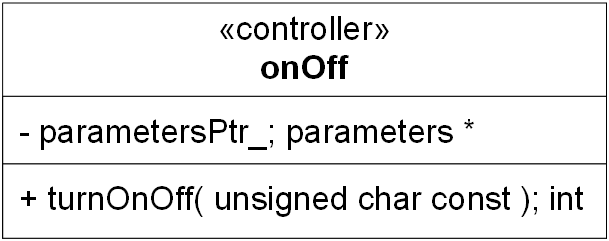
\includegraphics[scale=1.3]{filer/design/Klassediagrammer/sw_psoc_onOff}}
\caption{Klasse onOff}
\label{fig:sw_psoc_class_onOff}
\end{figure} 

{\centering
\textbf{onOff}\par
}
\textbf{Ansvar:} Kontrollerer hændelsesforløbet ifm. usecase 3. \

\verb+int turnOnOff( const unsigned char )+ \\
\textbf{Parametre:} En \verb+bool+ som angiver on = true, off = false \\
\textbf{Returværdi:} 0 ved succes ellers negativ i overenstemmelse med fejl-listen. \\
\textbf{Beskrivelse:} Skal sætte flaget \verb+active_+ i \verb+parameters+-objektet ud fra den modtagende parameter. Gyldige værdier er 0 og 1.\\

\begin{figure}[htbp] \centering
{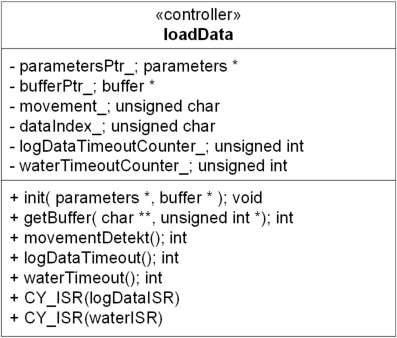
\includegraphics[scale=1.3]{filer/design/Klassediagrammer/sw_psoc_loadData}}
\caption{Klasse loadData}
\label{fig:sw_psoc_class_loadData}
\end{figure} 

{\centering
\textbf{loadData}\par
}
\textbf{Ansvar:} Kontrollerer hændelsesforløbet ifm. usecase 4. \

\verb+int getBuffer( char * buf, unsigned int len )+ \\
\textbf{Parametre:} Pointer til at skrive adressen til bufferen i og en længde. \\
\textbf{Returværdi:} 0 ved succes ellers negativ i overenstemmelse med fejl-listen. \\
\textbf{Beskrivelse:} Skal hente data fra \verb+buffer+-objektet og gemme det i parametrene \verb+buf+ og \verb+len+. Hvis \verb+active_+-flaget i \verb+parameters+ er sat, og målte værdier er uden for grænserne startes vanding ved at kalde \verb+water()+ i \verb+sensorPackage+-objektet. Her sættes også waterTimer i gang.\\

\verb+int movementDetekt( )+ \\
\textbf{Parametre:} Ingen. \\
\textbf{Returværdi:} 0 ved succes ellers negativ i overenstemmelse med fejl-listen. \\
\textbf{Beskrivelse:} Skal deaktiverer vanding ved at sætte \verb+active_+-flaget i \verb+parameters+-objektet til 0. Skal også starte en timer med udløb på 30 minutter. Skal sætte flaget \verb+movement_+ til 1, så der næste gang der gemmes data, registreres bevægelse. \\

\verb+int logDataTimeout( )+ \\
\textbf{Parametre:} Ingen. \\
\textbf{Returværdi:} 0 ved succes ellers negativ i overenstemmelse med fejl-listen. \\
\textbf{Beskrivelse:} Skal aflæses data fra \verb+sensorPackage+ og gemme disse i \verb+buffer+-objektet. Afhængig af \verb+movement_+-flaget, tilføjes passende \verb+char+ efter målt data i hht. dataprotokollen, og flaget sættes til 0. \\

\verb+int waterTimeout( )+ \\
\textbf{Parametre:} Ingen. \\
\textbf{Returværdi:} 0 ved succes ellers negativ i overenstemmelse med fejl-listen. \\
\textbf{Beskrivelse:} Skal aktivere muligheden for vanding ved at sætte \verb+active_+-flaget i \verb+parameters+-objektet til 1. \\
